\chapter{Introduction}
In this work, we simulate the phase space of a collisional dark matter fluid.
In order to follow the ideas and developments of the upcoming chapters, it is essential to understand some concepts and computational techniques.
In this chapter, we present all the necessary knowledge for the proper understanding of this work.
\section{Dark Matter}
Modern cosmology describes the universe as being composed of two fundamental types of energy: dark energy and matter\footnote{In relativity, mass and energy are equivalent.}, with dark energy being associate with a cosmological constant and matter being divided into two categories: dark matter and standard model matter\footnote{Which is very often called \tqt{Baryonic matter} due to Baryions being the largest fraction of this mass.}.
The energy density of the universe is $69\%$ dark energy and $31\%$ matter.

Standard model matter includes all the particles whose interactions can be properly described by the standard model, such as: Protons, Electrons, Atoms and naturally, any structure that they form, like Humans or Stars.
On the other hand, dark matter is all the matter we measure from astrophysical sources which cannot be explained by baryonic matter.
We know of the existence of dark matter entirely from astrophysical evidence, during this section we are going to do an historical review of such evidence.

\subsection{The Cluster Missing Mass Problem}
The traditional history of dark matter begins in the 1930s with the swiss astronomer Fritz Zwicky\cite{aHistory} \cite{tasiCline}, who noticed an unusually high velocity dispersion between the galaxies of the Coma Cluster.
To tackle the problem, Zwicky assumed that the Coma Cluster \tqt{had already reached a mechanically stationary state} \cite{englishZwicky} and such, the virial theorem could be applied.
By counting galaxies, along with assuming that matter is distributed uniformly in the cluster and using Hubble's estimate of the mean mass of a galaxy, Zwicky was able to estimate the potential energy of the Cluster.
Using his estimate of the visible mass and the virial theorem, Zwicky concluded that the velocity dispersion must be $\sqrt{\bar{v^2}} = 80$ km/s.
Nonetheless, the real measurement of the velocity dispersion was $\sqrt{\bar{v^2}} = 1000$ km/s, implying a virial mass about 400 times larger than the visible mass\footnote{This ratio is often called the mass-to-light ratio.}.
Zwicky called the discrepancy between the luminous matter (in the form of visible galaxies which could simply be counted) and the virial matter (obtained from the virial theorem and the high velocity dispersion of the cluster) \tqt{Dark Matter}. 

By the late 1950s similar calculations for different clusters had been published. Many of those calculations had very large values for the mass-to-light ratio\cite{schwarzschildSon}, which were consistent with the mass-to-light ratio calculated from the Coma Cluster. The problem of the missing mass seemed to appear in almost every large scale structure in the universe, and by the early 1970s astrophysicist had already disregarded hot gas\cite{meekins} and free hydrogen\cite{penzias} as explanations for the missing mass in Clusters. Nonetheless, it was still possible that the missing mass problem could be in fact solved by a more refined model of the cluster kinematics, because so far, the missing mass problem had only been observed on Clusters and large scale structures.

\subsection{Galaxy Rotation Curves}
A galaxy rotation curve plots the orbital velocity of stars in a galaxy versus their distance to the galaxy centre. These curves became important thanks to the work of the Indian astrophysics Subrahmanyan Chandrasekhar, who proved that the mutual interactions of stars were negligible, so a galaxy could be modeled as a non-interacting system of stars. Such modeling allows to obtain mass profiles from galaxy rotation curves. Now, due to photometric measurements, astrophysicist believed that most of the mass was overwhelmingly concentrated  in the galaxy centre, therefore, it was reasonable to model the galaxy similarly to the solar system. Consider a star in the galaxy disk with mass $m$ at a distance $r$ from the galaxy centre, given that we can disregard the interaction between starts, the sum of forces acting on the object is simply the gravitational attraction towards the galaxy centre:\\
\begin{equation}
m\frac{v^2}{r} = G \frac{mM}{r^2}
\end{equation}\\
With $M$ being the mass enclosed by the star orbit and $v$ being the orbital velocity of the star. Finally, the galaxy rotation curve for such galaxy will be given by:\\
\begin{equation}
v(r) = \sqrt{\frac{GM}{r}}
\end{equation}\\
Which means that for objects outside of the galaxy disk (but still under the influence of the galaxy gravitational pull), the enclosed mass will be constant regardless of the radius, and thus, the orbital velocity will be proportional to $r^{-1/2}$. With the advent of radio astronomy and the invention of the Image Tube Spectrograph, astronomers were able to measure orbital velocities way beyond the apparent end of the luminous galaxy disks, only to find that the orbital velocity did not decay proportionally to $r^{-1/2}$ but it stayed more or less constant\cite{h21Line} \cite{galactoDistance} \cite{veraFirst}. This behavior can be seen more easily in the figure \ref{galaxyCurve}
%Let's first state the basic properties of dark matter\cite{parnovskyCosmology}:

\begin{figure}[H]
    \centering
    %\includegraphics[width=10cm,height =7cm]{Diapositiva1.jpg}
    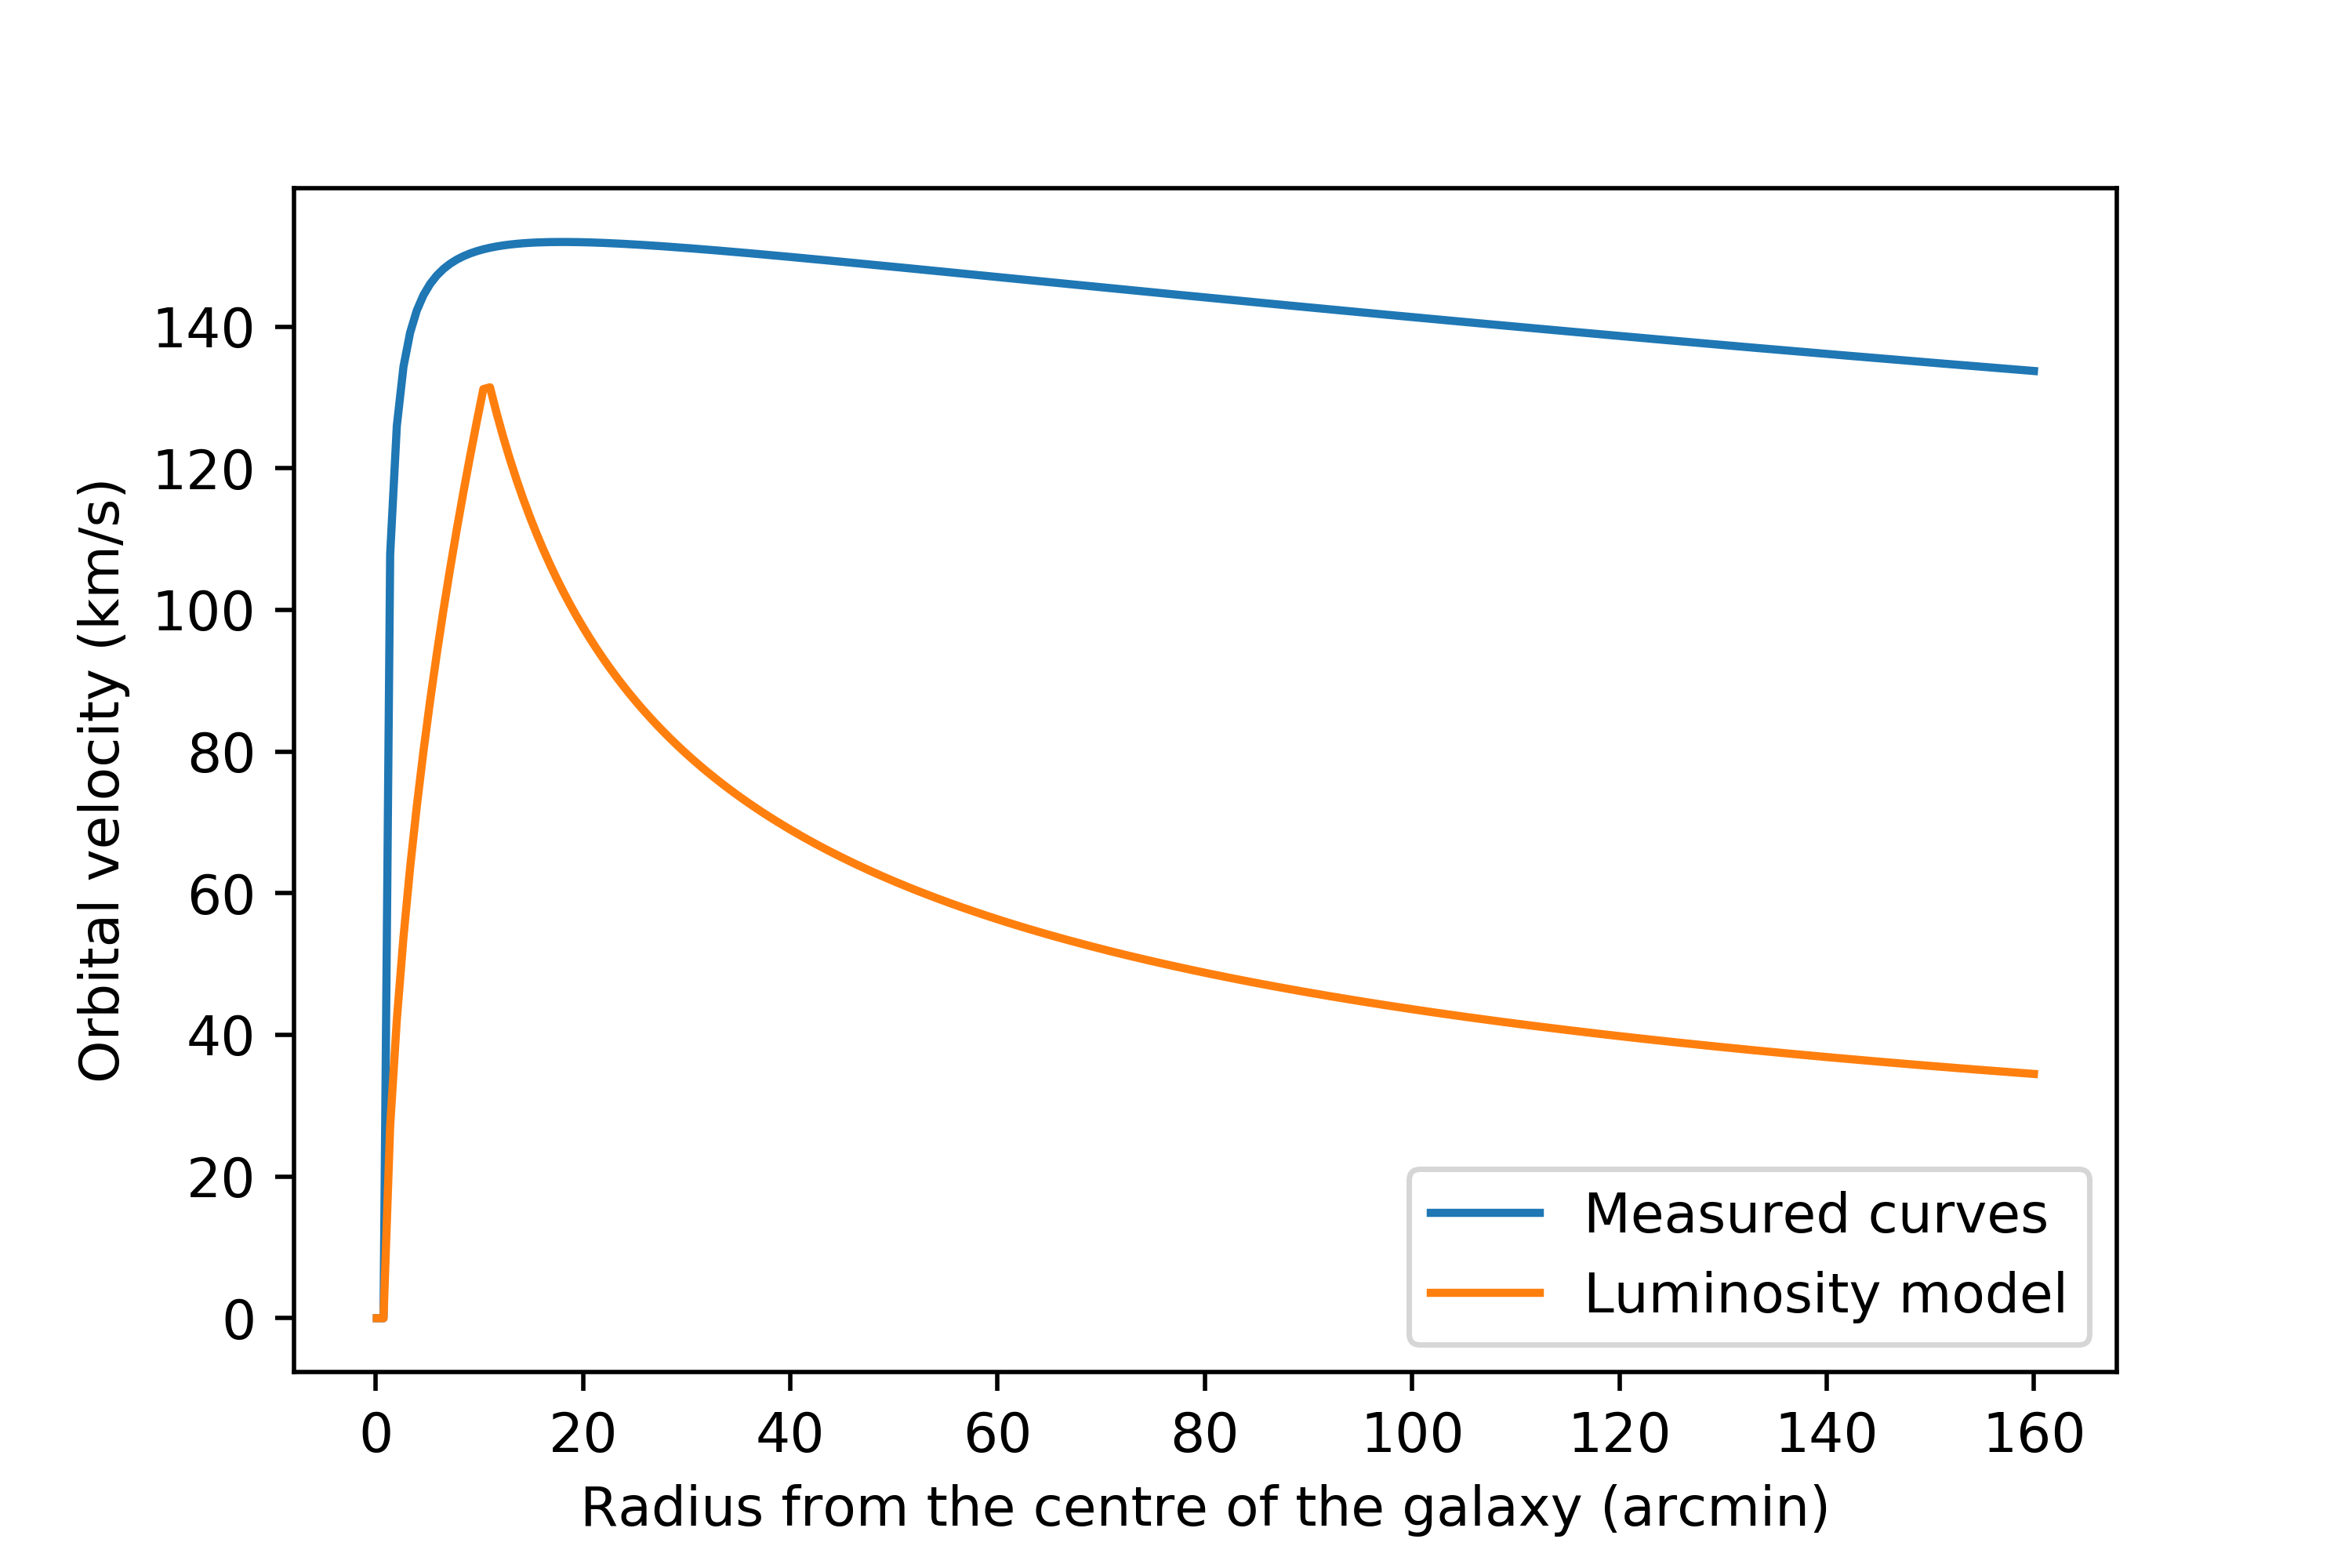
\includegraphics[scale=0.8]{imag/galaxyRotCurv.png}
    \caption{A comparison between the model from photometrical measurements and the curves measured. This curves are illustrative and do not correspond to a particular galaxy.}
    \label{galaxyCurve}
\end{figure}

This unexpected velocity profile implied a mass-to-light ratio that increased with distance and the existence of mass beyond the visible galactic disk\cite{theIsMassOutside}.
The overwhelming amount of high quality galaxy rotation curves measurements, let to the acceptance of the dark matter hypothesis in the astrophysical community.

Throughout the use of numerical simulations and the measurement of more galaxy rotation curves during the 1980s and the 1990s, it was concluded that the dark matter density in galaxies was well modeled by the Navarro-Frenk-White (NFW) profile\cite{FWN}\cite{mariangela}\\
\begin{equation}
\rho(r) = \frac{\rho_0}{r/r_s(1+r/r_s)^2}
\end{equation}


\subsection{The Bullet Cluster}
Galaxy clusters have three main constituents: dark matter, intracluster gas (which is almost in its entirety ionised hydrogen and helium), and the galaxy themselves.\cite{book:75345}


We can observe the intracluster baryonic matter in the x-ray band thanks to Bremsstrahlung radiation, therefore, by measuring photon count in astronomical images it is possible to map the baryonic gas distribution in a cluster.
In the case of dark matter, we infer its existence in clusters thanks to the work of Fritz Zwicky and the posterior work in the missing mass problem in galaxy clusters. By analyzing the gravitational lensing effect (in particular the gravitational \emph{weak} lensing effect), it is possible to map the mass distribution in a galaxy cluster. Given that most of the cluster mass is dark matter, weak lensing mapping ends up creating a map of the dark matter distribution in a galaxy cluster.
Lastly, we can observe galaxies in the visual and the infrared band.
They are the only component of a galaxy cluster that can be observed in the visual band.


The object Bullet Cluster (also known as 1E 0657-558) is the aftermath of the collision of two galaxy cluster.
Before the collision, each cluster had its own galaxies, baryonic gas and dark matter, and the center of mass of each constituent coincided with the center of mass of the whole cluster.
During the collision, each constituent reacts differently to the situation.
Galaxies, given that the occupy a minuscule volume in the cluster, are essentially collisionless. Two galaxy clusters can collide without any galaxy (or very little galaxies) colliding per se.






\section{Types of Dark Matter}

\section{The Boltzmann Equation}

\section{Lattice Automata and Lattice Boltzmann}

\section{BGK Approximation}
\label{bgk}
